% Self-contained research figure. Postulate R isolation, version 0.2.
% mu_std(x) = x/sqrt(1+x^2). Witnesses are drawn, not fitted.
\documentclass[tikz,border=6pt]{standalone}
\usepackage{pgfplots}
\pgfplotsset{compat=1.18}
\begin{document}
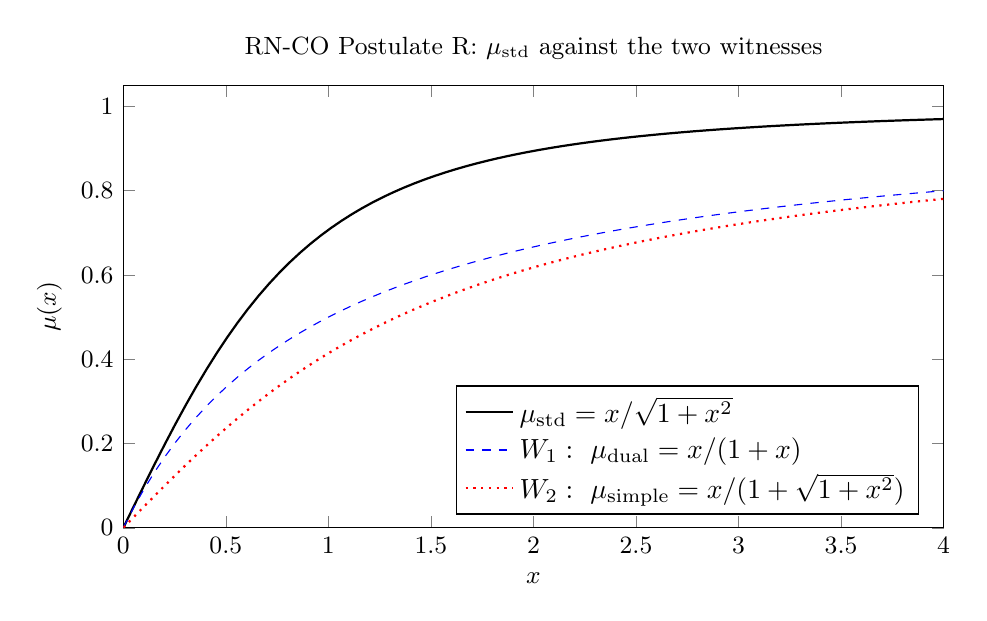
\begin{tikzpicture}
\begin{axis}[
  width=12cm, height=7.2cm,
  xlabel={$x$}, ylabel={$\mu(x)$},
  xmin=0, xmax=4, ymin=0, ymax=1.05,
  legend pos=south east,
  legend cell align=left,
  tick label style={font=\small},
  label style={font=\small},
  title style={font=\small},
  title={RN-CO Postulate R: $\mu_{\mathrm{std}}$ against the two witnesses},
  domain=0.001:4, samples=80,
]
\addplot[black, thick] {x/sqrt(1+x^2)};
\addlegendentry{$\mu_{\mathrm{std}}=x/\sqrt{1+x^{2}}$}
\addplot[blue, dashed] {x/(1+x)};
\addlegendentry{$W_1:\ \mu_{\mathrm{dual}}=x/(1+x)$}
\addplot[red, dotted, thick] {x/(1+sqrt(1+x^2))};
\addlegendentry{$W_2:\ \mu_{\mathrm{simple}}=x/(1+\sqrt{1+x^{2}})$}
\end{axis}
\end{tikzpicture}
\end{document}
